\subsection{Latency Overhead of NetShaper in Relation to Window \textit{W}}
\label{subsec:netshaper-evaluation-latency}

Finally, we evaluate how the choice of window $W$ impacts the latency observed by the client application.
We fix the request rate from wrk2 at 330k req/s.

As outlined in \Cref{subsec:netshaper-secret-independent-shaping-implementation}, NetShaper has a pre-profiled $T_{prep}$ and $T_{enq}$.
In our setup, $T_{prep} + T_{enq} = 10ms$.
As such, NetShaper always adds 10ms in each direction of shaping, resulting in a minimum round-trip latency of 20ms.
As shown in \Cref{fig:netshaper-eval-http-latency}, the average round-trip latency for the client application is directly dependent on the window $W$.
The high variance in the latency is caused by the window $W$, as the request that arrives at the start of window $W$ will wait for the entire duration of $W$, but the request that arrives at the end of $W$ will be almost immediately sent out.

\begin{figure}[!htb]
    \centering
    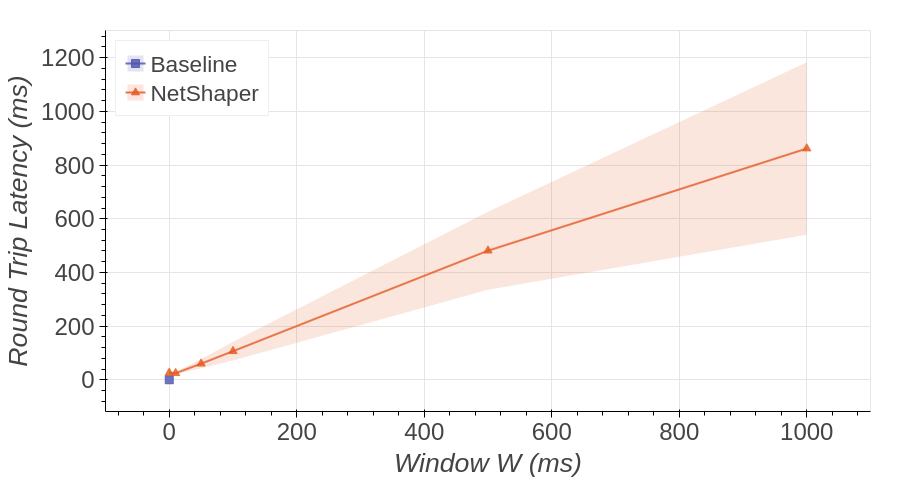
\includegraphics[width=\columnwidth]{figures/netshaper/evaluation/http_latency.png}
    \caption{Latency vs $W$. The baseline has only measurement as it does not have $W$, which is a parameter for NetShaper.
    NetShaper's latency increases with $W$.
    The variation in latency (shaded region) is due to the varying arrival time of requests or responses within $W$.}
    \label{fig:netshaper-eval-http-latency}
\end{figure}